\documentclass{beamer}

\usepackage[T1]{fontenc}
\usepackage[utf8]{inputenc}
\usepackage[frenchb]{babel}
\usepackage{eurosym}

\usepackage{graphicx}


\newcommand\host{{\it host}\,}
\newcommand\device{{\it device}\,}


% --------- BEGIN STYLE BEAMER ---------
\usetheme{Madrid}
\definecolor{ECNBleu}{HTML}{102648}
\definecolor{ECNJaune}{HTML}{FAB600}

\setbeamercolor{frametitle}{bg=ECNBleu,fg=white} %le titre de la frame, en haut
\setbeamercolor{title in head/foot}{bg=ECNJaune,fg=ECNBleu} %barre bas, milieu
\setbeamercolor{author in head/foot}{bg=ECNBleu,fg=ECNJaune} %barre bas, gauche
\setbeamercolor{date in head/foot}{bg=ECNBleu,fg=ECNJaune} %barre bas, droit
\setbeamercolor{section in head/foot}{bg=ECNJaune,fg=ECNBleu} %haut gauche
\setbeamercolor{subsection in head/foot}{bg=ECNBleu,fg=ECNBleu} %haut droite
\setbeamercolor{title}{bg=ECNBleu,fg=white}
\setbeamercolor{block title}{fg=white,bg=ECNBleu}

%\setbeamercolor{normal text}{bg=IUTBleuFonce} %texte
\setbeamercolor{item}{bg=ECNBleu}
\setbeamercolor{subitem}{bg=ECNJaune}
\setbeamercolor{description item}{fg=couleurEmph}
\setbeamercolor{section in toc}{fg=ECNBleu}
%\setbeamercolor{subsubitem}{bg=IUTBleuFonce}

%structure (eq emph dans beamer)
\setbeamercolor{emph}{fg=couleurEmph}
% ----------------------------

\usepackage{listings}

\lstdefinestyle{customc}{
  belowcaptionskip=1\baselineskip,
  breaklines=true,
  frame=L,
  xleftmargin=\parindent,
  language=C,
  showstringspaces=false,
  basicstyle=\tiny\ttfamily,
  keywordstyle=\bfseries\color{green!40!black},
  commentstyle=\itshape\color{purple!40!black},
  identifierstyle=\color{blue},
  stringstyle=\color{orange},
}

\lstset{escapechar=@,style=customc}

\newenvironment<>{questionblock}[1]{%
\setbeamercolor{block title}{bg=ECNJaune,fg=ECNBleu}%
\begin{block}#2{#1}}{\end{block}}

\title[GPGPU]{Programmation sur Processeur Graphique}

\subtitle[\ldots]{
---\\Partie 3 : Kernel à plusieurs dimensions}
\author[P.-E. Hladik]{Pierre-Emmanuel Hladik\\\tiny pierre-emmanuel.hladik@ec-nantes.fr}
\institute[Centrale Nantes]{}
\date{\today}

\begin{document}

 \frame{\titlepage}

%%%%%%%%%%%%%%%%%%%%%%%%%%%
%%%%%%%%%%%%%%%%%%%%%%%%%%%
\section{Introduction à la programmation parallèle}
\section{Allocation des données et exécution d'un kernel}
\section{Kernel à plusieurs dimensions}
%%%%%%%%%%%%%%%%%%%%%%%%%%%
\begin{frame}{Plan}
\tableofcontents[sections={1-4}, currentsection, hideothersubsections]
\end{frame}
%%%%%%%%%%%%%%%%%%%%%%%%%%%

%%%%%%%%%%%%%%%%%%%%%%%%%%
\begin{frame}[plain]
\frametitle{blockIdx et threadIdx}
      \begin{block}{}
	\begin{itemize}
		\item les index de block et de thread sont des variables à trois dimensions
		\item cela simplifie les adresses mémoires quand on travaille avec des données multidimentionelles (image, volumes, etc.)
	\end{itemize}
      \center
	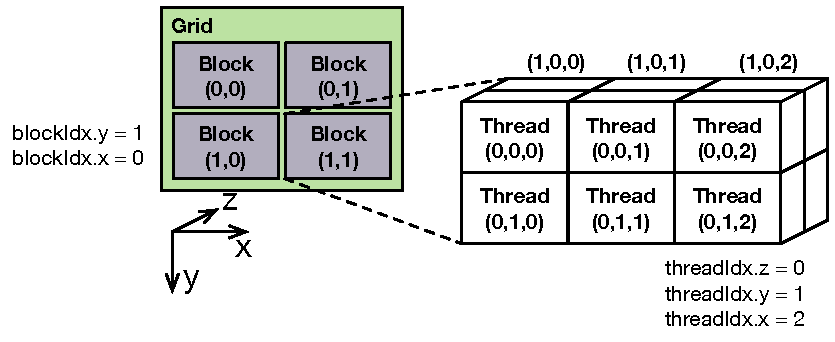
\includegraphics[scale=0.7]{./figures-pdf/indexDim}
	\end{block}  
\end{frame}
%%%%%%%%%%%%%%%%%%%%%%%%%%
\begin{frame}[plain,fragile]
\frametitle{Exemple : niveau de gris pour une image en 2D}
      \center
	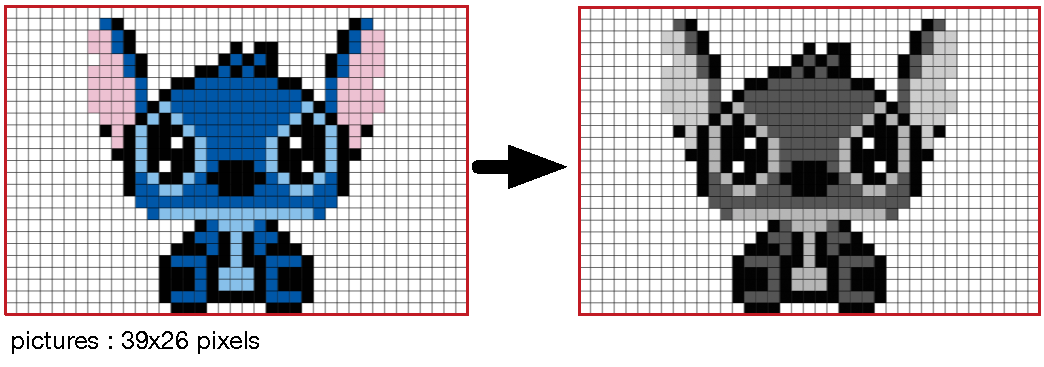
\includegraphics[scale=0.6]{./figures-pdf/stitch}
\end{frame}
%%%%%%%%%%%%%%%%%%%%%%%%%%
\begin{frame}[plain,fragile]
\frametitle{Représentation RVB d'une image et niveau de gris}
      \begin{block}{}
	\begin{itemize}
		\item Pour chaque pixel $(r,v,b)$ en position $(i,j)$ :
		$$grayPixel[i,j] = 0.21\times r + 0.71\times v + 0.07\times b $$
		\item C'est l'équivalent du produit scalaire $(r,v,b) \cdot (0.21, 0.71, 0.07)$ avec des constantes spécifiques à l'espace RVB
	\end{itemize}
      \center
	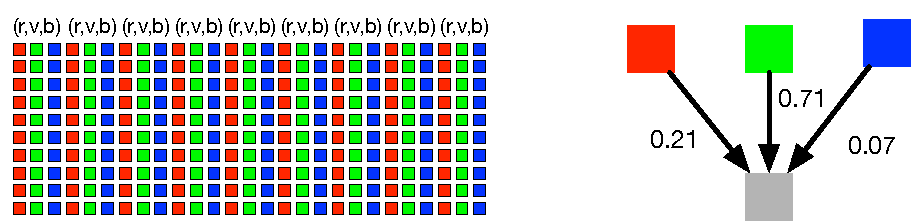
\includegraphics[scale=0.7]{./figures-pdf/rvb}
	\end{block}  
\end{frame}
%%%%%%%%%%%%%%%%%%%%%%%%%%
\begin{frame}[plain,fragile]
\frametitle{{\it Représentation des tableaux : Row-Major Order} en C/C++}
      \center
	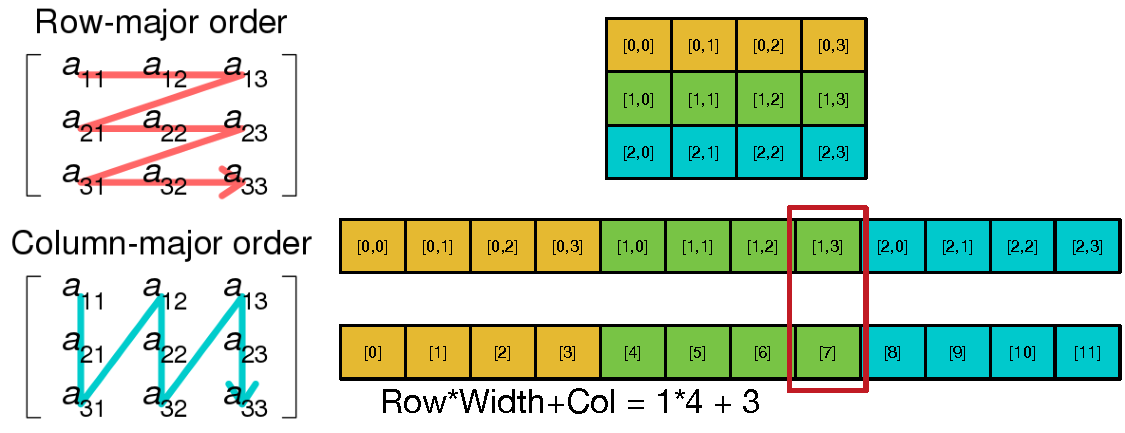
\includegraphics[scale=0.55]{./figures-pdf/row-major}
\end{frame}
%%%%%%%%%%%%%%%%%%%%%%%%%%
\begin{frame}[plain,fragile]
\frametitle{Pseudo-algo CPU}

	  \begin{lstlisting}[language=C]
for ii from 0 to height do
  for jj from 0 to width do
    idx = ii * width + jj
    r = input[3*idx]
    g = input[3*idx + 1]
    b = input[3*idx + 2]
    grayImage[idx] = (0.21*r + 0.71*g + 0.07*b)
  end
end    
 	  \end{lstlisting}
\end{frame}


%%%%%%%%%%%%%%%%%%%%%%%%%%
\begin{frame}[plain,fragile]
\frametitle{Création de la {\it grid}}
      \center
	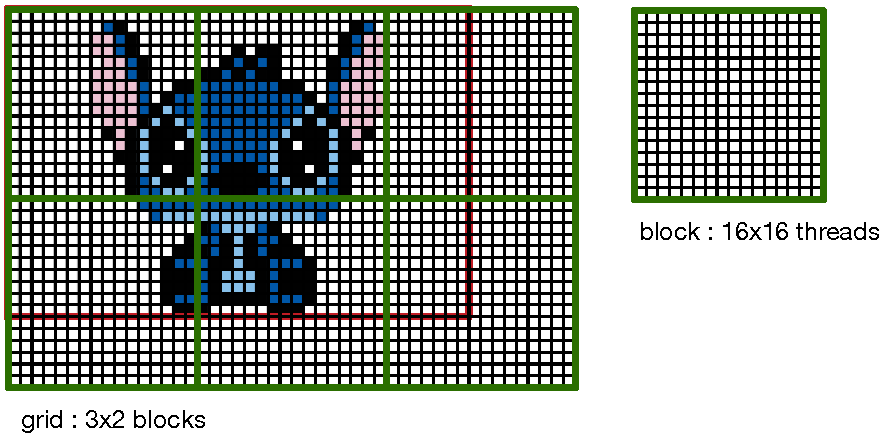
\includegraphics[scale=0.7]{./figures-pdf/grid}
\end{frame}
%%%%%%%%%%%%%%%%%%%%%%%%%%
\begin{frame}[plain,fragile]
\frametitle{Kernel}
	  \begin{lstlisting}[language=C]
#define CHANNELS 3 // we have 3 channels corresponding to RGB
// The input image is encoded as unsigned characters [0, 255]
__global__ 
void colorConvert(unsigned char * grayImage, // output image
		  unsigned char * rgbImage, // input image
                  int width, 
                  int height) {
                  
  int x = threadIdx.x + blockIdx.x * blockDim.x; // Col
  int y = threadIdx.y + blockIdx.y * blockDim.y; // Row

  if (x < width && y < height) {
    // get 1D coordinate for the grayscale image
    int grayOffset = y*width + x;
    
    // one can think of the RGB image having
    // CHANNEL times columns than the gray scale image
    int rgbOffset = grayOffset*CHANNELS;
    unsigned char r = rgbImage[rgbOffset    ]; // red value for pixel
    unsigned char g = rgbImage[rgbOffset + 2]; // green value for pixel
    unsigned char b = rgbImage[rgbOffset + 3]; // blue value for pixel

    // perform the rescaling and store it
    // We multiply by floating point constants
    grayImage[grayOffset] = 0.21f*r + 0.71f*g + 0.07f*b;
  }
}
   	  \end{lstlisting}
\end{frame}
%%%%%%%%%%%%%%%%%%%%%%%%%%
\begin{frame}[plain,fragile]
\frametitle{Création de la {\it grid}}
      \center
	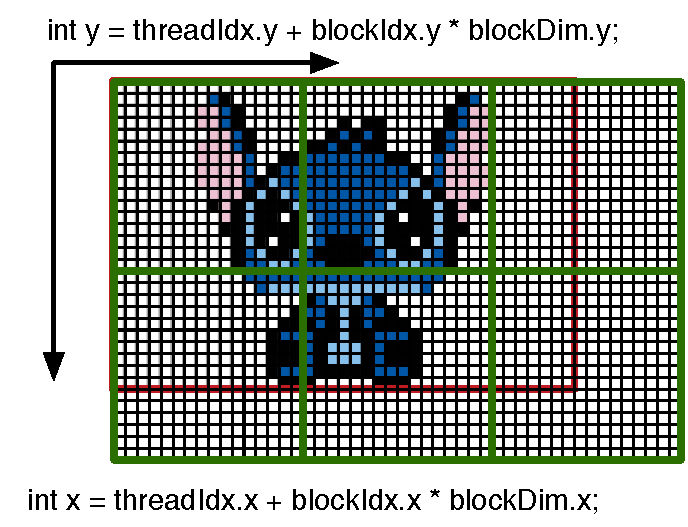
\includegraphics[scale=0.7]{./figures-pdf/x_y}
\end{frame}
%%%%%%%%%%%%%%%%%%%%%%%%%%
\begin{frame}[plain,fragile]
\frametitle{Code de l'{\it host} pour lancer l'exécution}
	  \begin{lstlisting}[language=C]
// assume that the picture is m X n, 
// m pixels in y dimension and n pixels in x dimension
// input d_Pin has been allocated on and copied to device
// output d_Pout has been allocated on device
...
dim3 dimGrid((n-1)/16 + 1, (m-1)/16+1, 1);
dim3 dimBlock(16, 16, 1);
colorConvert<<<dimGrid, dimBlock>>>(grayImage, rgbImage, width, height);
...
   	  \end{lstlisting}
\end{frame}
%%%%%%%%%%%%%%%%%%%%%%%%%%
\begin{frame}[plain,fragile]
\frametitle{Couverture de l'image par les blocs}
      \begin{block}{}

 Tous les threads dans un bloc n'ont pas le même chemin dans leur flot de contrôle.
      \center
	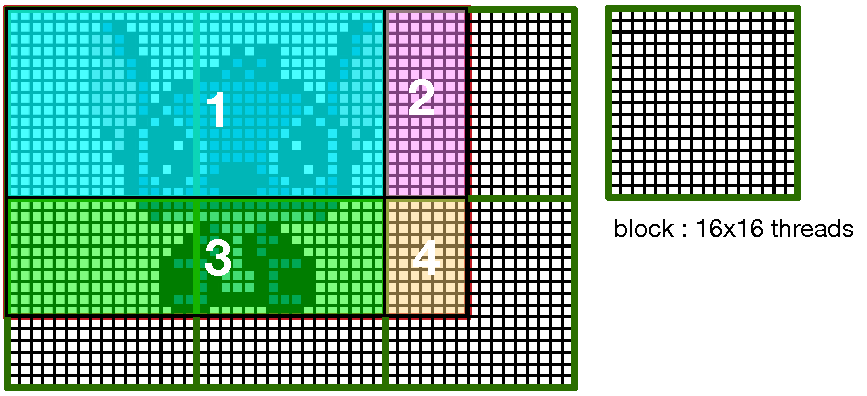
\includegraphics[scale=0.7]{./figures-pdf/stitch_blocs}
	\end{block}  
\end{frame}

%%%%%%%%%%%%%%%%%%%%%%%%%%
\begin{frame}[plain]
\frametitle{Un peu de pratique avec le TD3}

\begin{block}{Objectifs}
\begin{itemize}
	\item Utilisation d'un kernel à plusieurs dimensions
	\item Gestion d'une méthode dans une structure sur un {\it device}
\end{itemize}
\end{block}
\end{frame}
%%%%%%%%%%%%%%%%%%%%%%%%%%

\end{document}